\documentclass{article}
\usepackage{tikz}
\usepackage{amsmath}
\usepackage{tkz-euclide}
\begin{document}
\tikzset{font=\scriptsize}
\section{TEOREMA DE PICK 1.0}
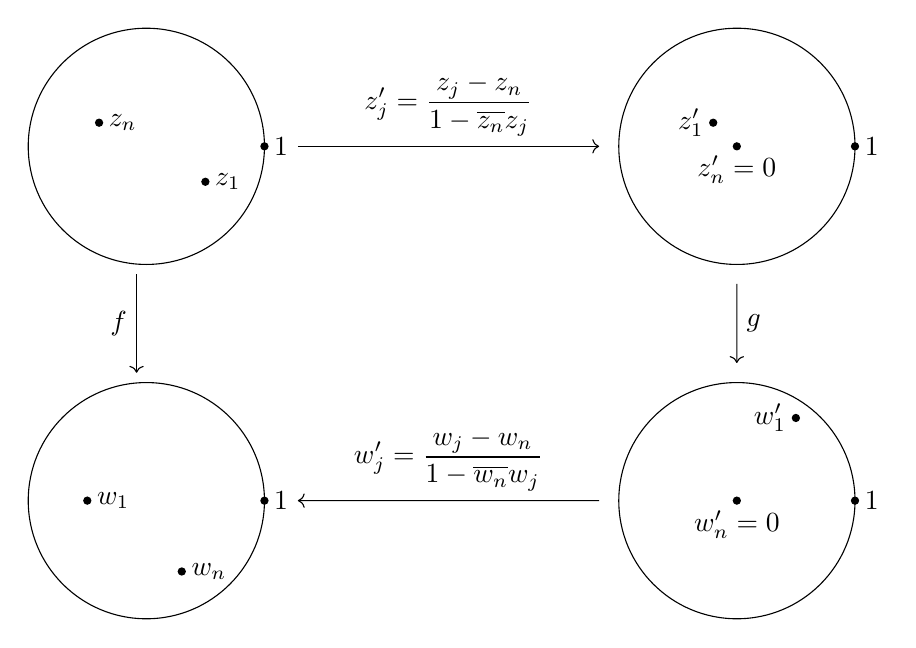
\begin{tikzpicture}[scale = 1.5]
    \draw (0,0) circle [radius=1cm];
    \coordinate[label=right:$z_1$] (B) at (0.5, -0.3);
    \coordinate[label=right:$z_n$] (C) at (-0.4, 0.2);
    \node[right, fill=white] (A) at (1,0) {1};
    \node[left] (H) at (0,-1) {\space};
    \fill[black] (1,0) circle (1pt);
    \fill[black] (B) circle (1pt);
    \fill[black] (C) circle (1pt);

    \draw (5,0) circle [radius=1cm];
    \coordinate[label=left:$z'_1$] (D) at (4.8, 0.2);
    \coordinate[label=below:{$z'_n=0$}] (E) at (5, 0);
    \node[right, fill=white] (F) at (6,0) {1};
    \node[left] (G) at (4,0) {\space};
    \node[below] (R) at (5,-1) {\space};
    \fill[black] (6,0) circle (1pt);
    \fill[black] (D) circle (1pt);
    \fill[black] (E) circle (1pt);

    \draw[->] (A) -- (G) node[pos=0.5,above] {$\displaystyle z'_j=\frac{z_j-z_n}{1-\overline{z_n}z_j}$};

    \draw (0,-3) circle [radius=1cm];
    \coordinate[label=right:$w_1$] (I) at (-.5, -3);
    \coordinate[label=right:$w_n$] (J) at (0.3, -3.6);
    \node[right, fill=white] (K) at (1,-3) {1};
    \node[left] (L) at (0,-2) {\space};
    \fill[black] (1,-3) circle (1pt);
    \fill[black] (I) circle (1pt);
    \fill[black] (J) circle (1pt);

    \draw[->] (H) -- (L) node[pos=0.5,left] {$\displaystyle f$};

    \draw (5,-3) circle [radius=1cm];
    \coordinate[label=left:$w'_1$] (M) at (5.5, -2.3);
    \coordinate[label=below:{$w'_n=0$}] (N) at (5, -3);
    \node[right, fill=white] (O) at (6,-3) {1};
    \node[left] (P) at (4,-3) {\space};
    \node[above] (Q) at (5,-2) {\space};
    \fill[black] (6,-3) circle (1pt);
    \fill[black] (M) circle (1pt);
    \fill[black] (N) circle (1pt);

    \draw[->] (P) -- (K) node[pos=0.5,above] {$\displaystyle w'_j=\frac{w_j-w_n}{1-\overline{w_n}w_j}$};
    \draw[->] (R) -- (Q) node[pos=0.5,right] {$\displaystyle g$};

\end{tikzpicture}

\newpage
\section{TEOREMA DE PICK 1.5}
\usetikzlibrary{arrows}
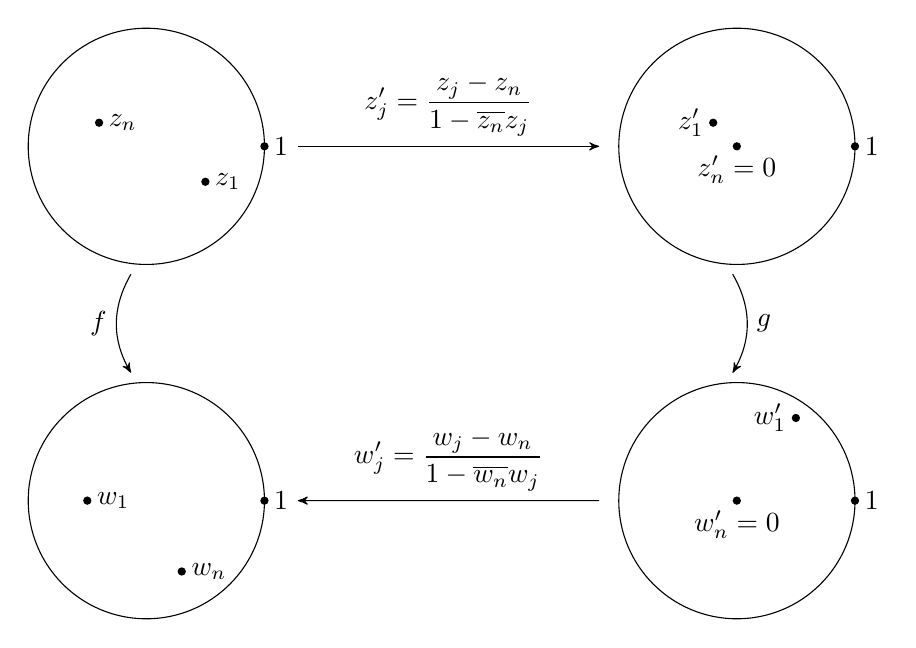
\begin{tikzpicture}[scale = 1.5,->,>=stealth']
    \draw (0,0) circle [radius=1cm];
    \coordinate[label=right:{$z_1$}] (B) at (0.5, -0.3);
    \coordinate[label=right:{$z_n$}] (C) at (-0.4, 0.2);
    \node[right, fill=white] (A) at (1,0) {1};
    \node[left] (H) at (0,-1) {\space};
    \fill[black] (1,0) circle (1pt);
    \fill[black] (B) circle (1pt);
    \fill[black] (C) circle (1pt);

    \draw (5,0) circle [radius=1cm];
    \coordinate[label=left:$z'_1$] (D) at (4.8, 0.2);
    \coordinate[label=below:{$z'_n=0$}] (E) at (5, 0);
    \node[right, fill=white] (F) at (6,0) {1};
    \node[left] (G) at (4,0) {\space};
    \node[left] (R) at (5,-1) {\space};
    \fill[black] (6,0) circle (1pt);
    \fill[black] (D) circle (1pt);
    \fill[black] (E) circle (1pt);


    \draw (0,-3) circle [radius=1cm];
    \coordinate[label=right:$w_1$] (I) at (-.5, -3);
    \coordinate[label=right:$w_n$] (J) at (0.3, -3.6);
    \node[right, fill=white] (K) at (1,-3) {1};
    \node[left] (L) at (0,-2) {\space};
    \fill[black] (1,-3) circle (1pt);
    \fill[black] (I) circle (1pt);
    \fill[black] (J) circle (1pt);


    \draw (5,-3) circle [radius=1cm];
    \coordinate[label=left:$w'_1$] (M) at (5.5, -2.3);
    \coordinate[label=below:{$w'_n=0$}] (N) at (5, -3);
    \node[right, fill=white] (O) at (6,-3) {1};
    \node[left] (P) at (4,-3) {\space};
    \node[left] (Q) at (5,-2) {\space};
    \fill[black] (6,-3) circle (1pt);
    \fill[black] (M) circle (1pt);
    \fill[black] (N) circle (1pt);

 
    \path[]
    (A) edge node [pos=.5, above] {$\displaystyle z'_j=\frac{z_j-z_n}{1-\overline{z_n}z_j}$} (G)
    (H) edge[bend right] node [left] {$f$} (L)
    (P) edge node [pos=.5, above] {$\displaystyle w'_j=\frac{w_j-w_n}{1-\overline{w_n}w_j}$} (K)
    (R) edge[bend left] node [right] {$g$} (Q);
\end{tikzpicture}

\newpage
\section{TEOREMA DE PICK 2.0}
\usetikzlibrary{arrows}
\usetikzlibrary{calc}
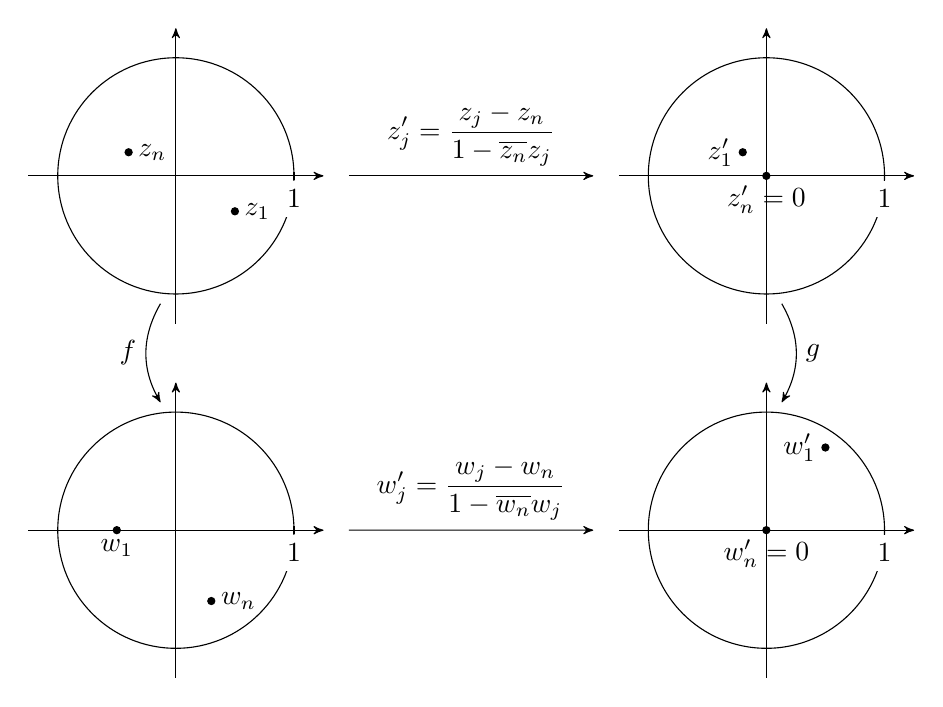
\begin{tikzpicture}[scale = 1.5,>=stealth']
    \draw (0,0) circle [radius=1cm];
    \draw[->] (-1.25,0) -- (1.25,0) coordinate (x axis);
    \draw[->] (0, -1.25) -- (0, 1.25) coordinate (y axis);
    \draw (1 cm,1pt) -- (1 cm,-1pt) node[anchor=north,fill=white] {1};
    \coordinate[label=right:$z_1$] (B) at (0.5, -0.3);
    \coordinate[label=right:$z_n$] (C) at (-0.4, 0.2);
    \node[right] (A) at (1.3,0) {\space};
    \node[left] (H) at (0,-1) {\space};
    \fill[black] (B) circle (1pt);
    \fill[black] (C) circle (1pt);

    \draw (5,0) circle [radius=1cm];
    \draw[->] (3.75,0) -- (6.25,0) coordinate (x axis);
    \draw[->] (5, -1.25) -- (5, 1.25) coordinate (y axis);
    \draw (6 cm,1pt) -- (6 cm,-1pt) node[anchor=north,fill=white] {1};
    \coordinate[label=left:$z'_1$] (D) at (4.8, 0.2);
    \coordinate[label=below:{$z'_n=0$}] (E) at (5, 0);
    \node[left] (G) at (3.7,0) {\space};
    \node[right] (R) at (5,-1) {\space};
    \fill[black] (D) circle (1pt);
    \fill[black] (E) circle (1pt);


    \draw (0,-3) circle [radius=1cm];
    \draw[->] (-1.25,-3) -- (1.25,-3) coordinate (x axis);
    \draw[->] (0, -4.25) -- (0, -1.75) coordinate (y axis);
    \coordinate (aux1) at (1, -3);
    \draw ($(aux1) + (0, 1 pt)$) -- ($(aux1) + (0,-1pt)$) node[anchor=north,fill=white] {1};
    \coordinate[label=below:$w_1$] (I) at (-.5, -3);
    \coordinate[label=right:$w_n$] (J) at (0.3, -3.6);
    \node[right, fill=white] (K) at (1.3,-3) {\space};
    \node[left] (L) at (0,-2) {\space};
    \fill[black] (I) circle (1pt);
    \fill[black] (J) circle (1pt);


    \draw (5,-3) circle [radius=1cm];
    \draw[->] (3.75,-3) -- (6.25,-3) coordinate (x axis);
    \draw[->] (5, -4.25) -- (5, -1.75) coordinate (y axis);
    \coordinate (aux2) at (6, -3);
    \draw ($(aux2) + (0, 1 pt)$) -- ($(aux2) + (0,-1pt)$) node[anchor=north,fill=white] {1};
    \coordinate[label=left:$w'_1$] (M) at (5.5, -2.3);
    \coordinate[label=below:{$w'_n=0$}] (N) at (5, -3);
    \node[left] (P) at (3.7,-3) {\space};
    \node[right] (Q) at (5,-2) {\space};
    \fill[black] (M) circle (1pt);
    \fill[black] (N) circle (1pt);

 
    \path[->]
    (A) edge node [pos=.5, above] {$\displaystyle z'_j=\frac{z_j-z_n}{1-\overline{z_n}z_j}$} (G)
    (H) edge[bend right] node [left] {$f$} (L)
    (K) edge node [pos=.5, above] {$\displaystyle w'_j=\frac{w_j-w_n}{1-\overline{w_n}w_j}$} (P)
    (R) edge[bend left] node [right] {$g$} (Q);
\end{tikzpicture}


\newpage
\section{Lema Previ al Problema 1.0}
\usetikzlibrary{arrows}
\usetikzlibrary{calc}
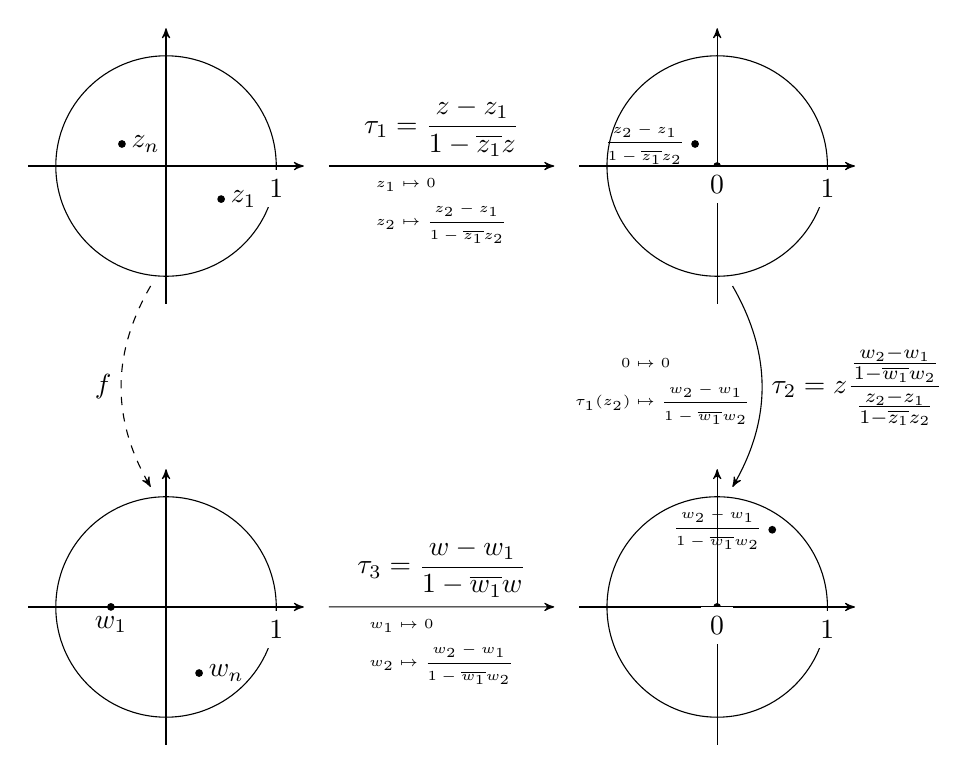
\begin{tikzpicture}[scale = 1.4,>=stealth']
    \draw (0,0) circle [radius=1cm];
    \draw[->] (-1.25,0) -- (1.25,0) coordinate (x axis);
    \draw[->] (0, -1.25) -- (0, 1.25) coordinate (y axis);
    \draw (1 cm,1pt) -- (1 cm,-1pt) node[anchor=north,fill=white] {1};
    \coordinate[label=right:$z_1$] (B) at (0.5, -0.3);
    \coordinate[label=right:$z_n$] (C) at (-0.4, 0.2);
    \node[right] (A) at (1.3,0) {\space};
    \node[left] (H) at (0,-1) {\space};
    \fill[black] (B) circle (1pt);
    \fill[black] (C) circle (1pt);

    \draw (5,0) circle [radius=1cm];
    \draw[->] (3.75,0) -- (6.25,0) coordinate (x axis);
    \draw[->] (5, -1.25) -- (5, 1.25) coordinate (y axis);
    \draw (6 cm,1pt) -- (6 cm,-1pt) node[anchor=north,fill=white] {1};
    \coordinate[label=left:{\tiny$\displaystyle\frac{z_2-z_1}{1-\overline{z_1}z_2}$}] (D) at (4.8, 0.2);
    \coordinate (E) at (5, 0);
    \node[left] (G) at (3.7,0) {\space};
    \node[right] (R) at (5,-1) {\space};
    \fill[black] (D) circle (1pt);
    \fill[black] (E) circle (1pt) node[anchor=north, fill=white] {$0$};


    \draw (0,-4) circle [radius=1cm];
    \draw[->] (-1.25,-4) -- (1.25,-4) coordinate (x axis);
    \draw[->] (0, -5.25) -- (0, -2.75) coordinate (y axis);
    \coordinate (aux1) at (1, -4);
    \draw ($(aux1) + (0, 1 pt)$) -- ($(aux1) + (0,-1pt)$) node[anchor=north,fill=white] {1};
    \coordinate[label=below:$w_1$] (I) at (-.5, -4);
    \coordinate[label=right:$w_n$] (J) at (0.3, -4.6);
    \node[right, fill=white] (K) at (1.3,-4) {\space};
    \node[left] (L) at (0,-3) {\space};
    \fill[black] (I) circle (1pt);
    \fill[black] (J) circle (1pt);


    \draw (5,-4) circle [radius=1cm];
    \draw[->] (3.75,-4) -- (6.25,-4) coordinate (x axis);
    \draw[->] (5, -5.25) -- (5, -2.75) coordinate (y axis);
    \coordinate (aux2) at (6, -4);
    \draw ($(aux2) + (0, 1 pt)$) -- ($(aux2) + (0,-1pt)$) node[anchor=north,fill=white] {1};
    \coordinate[label=left:{\tiny$\displaystyle\frac{w_2-w_1}{1-\overline{w_1}w_2} $}] (M) at (5.5, -3.3);
    \coordinate (N)  at (5, -4);
    \node[left] (P) at (3.7,-4) {\space};
    \node[right] (Q) at (5,-3) {\space};
    \fill[black] (M) circle (1pt);
    \fill[black] (N) circle (1pt) node[anchor=north, fill=white] {$0$};


    \path[->]
    (A) edge node [pos=.5, above] {$\displaystyle \tau_1=\frac{z-z_1}{1-\overline{z_1}z}$} node[pos=.5, below] {\tiny$\displaystyle\begin{aligned} z_1&\mapsto 0 \\
        z_2 &\mapsto  \frac{z_2-z_1}{1-\overline{z_1}z_2} \end{aligned}$ } (G)
    (H) edge[bend right, dashed] node [left] {$f$} (L)
    (K) edge node [pos=.5, above] {$\displaystyle \tau_3=\frac{w-w_1}{1-\overline{w_1}w}$} node[pos=.5, below] {\tiny$\displaystyle\begin{aligned} w_1&\mapsto 0 \\
        w_2 &\mapsto  \frac{w_2-w_1}{1-\overline{w_1}w_2} \end{aligned}$ } (P)
    (R) edge[bend left] node [right] {$\displaystyle \tau _{2} =z\frac{\frac{w_{2} -w_{1}}{1-\overline{w_{1}} w_{2}}}{\frac{z_{2} -z_{1}}{1-\overline{z_{1}} z_{2}}}$} node[pos=0.3, below, xshift=-1.2cm] {\tiny$\displaystyle\begin{aligned} 0&\mapsto 0 \\
         \tau_1(z_2) &\mapsto  \frac{w_2-w_1}{1-\overline{w_1}w_2}\end{aligned}$ }(Q);
\end{tikzpicture}



\newpage
\section{Esfera Riemann 1.0}
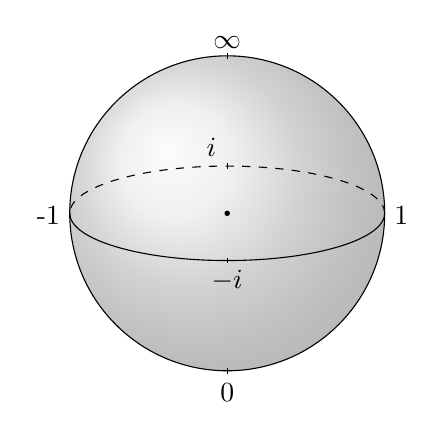
\begin{tikzpicture}
    \coordinate (aux) at (0, -2);
    \coordinate (aux2) at (0, 2);
    \shade[ball color = gray!40, opacity = 0.4] (0,0) circle (2cm);
    \draw (0,0) circle (2cm);
    \draw (-2,0) arc (180:360:2 and 0.6) node[pos=.5] (A) {};
    \draw ($(A) + (0, 1pt)$) -- ($(A) + (0,-1pt)$) node [pos=.5, below]{$-i$};
    \draw[dashed] (2,0) arc (0:180:2 and 0.6) node[pos=.5] (B) {};
    \draw ($(B) + (0, 1.1pt)$) -- ($(B) + (0,-1.1pt)$) node [pos=.5, above, xshift=-2mm]{$i$};
    \fill[fill=black] (0,0) circle (1pt);
    \draw (2 cm,1pt) -- (2 cm,-1pt) node[anchor=west] {1};
    \draw (-2 ,1pt) -- (-2,-1pt) node[anchor=east] {-1};
    \draw ($(aux) + (0,1pt)$)-- ($(aux) + (0,-1pt)$) node[anchor=north] {0};
    \draw ($(aux2) + (0,1pt)$)-- ($(aux2) + (0,-1pt)$) node[anchor=south] {$\infty$};
  \end{tikzpicture}
\newpage
\section{Esfera Riemann 1.5}

  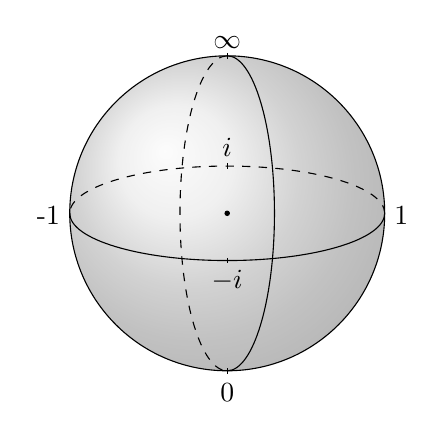
\begin{tikzpicture}
    \coordinate (aux) at (0, -2);
    \coordinate (aux2) at (0, 2);
    \shade[ball color = gray!40, opacity = 0.4] (0,0) circle (2cm);
    \draw (0,0) circle (2cm);
    \draw (-2,0) arc (180:360:2 and 0.6) node[pos=.5] (A) {};
    \draw ($(A) + (0, 1pt)$) -- ($(A) + (0,-1pt)$) node [pos=.5, below]{$-i$};
    \draw[dashed] (2,0) arc (0:180:2 and 0.6) node[pos=.5] (B) {};
    \draw ($(B) + (0, 1.1pt)$) -- ($(B) + (0,-1.1pt)$) node [pos=.5, above]{$i$};
    \draw[cm={cos(90) ,-sin(90) ,sin(90) ,cos(90) ,(0 cm,0 cm)}] (2,0) arc (0:180:2 and 0.6);
    \draw[dashed,cm={cos(90) ,-sin(90) ,sin(90) ,cos(90) ,(0 cm,0 cm)} ] (-2,0) arc (180:360:2 and 0.6);
    \fill[fill=black] (0,0) circle (1pt);
    \draw (2 cm,1pt) -- (2 cm,-1pt) node[anchor=west] {1};
    \draw (-2 ,1pt) -- (-2,-1pt) node[anchor=east] {-1};
    \draw ($(aux) + (0,1pt)$)-- ($(aux) + (0,-1pt)$) node[anchor=north] {0};
    \draw ($(aux2) + (0,1pt)$)-- ($(aux2) + (0,-1pt)$) node[anchor=south] {$\infty$};
  \end{tikzpicture}

  \newpage
\section{Esfera Riemann 2.0}

  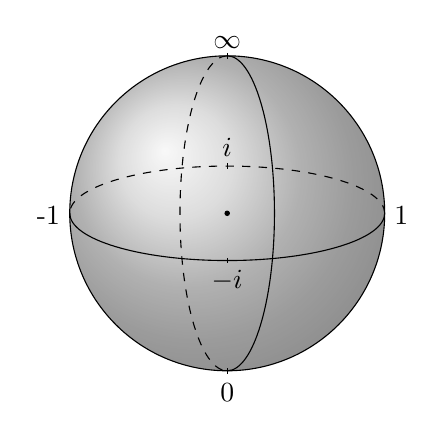
\begin{tikzpicture}
    \coordinate (aux) at (0, -2);
    \coordinate (aux2) at (0, 2);
    \shade[ball color = gray!60, opacity = 0.6] (0,0) circle (2cm);
    \draw (0,0) circle (2cm);
    \draw (-2,0) arc (180:360:2 and 0.6) node[pos=.5] (A) {};
    \draw ($(A) + (0, 1pt)$) -- ($(A) + (0,-1pt)$) node [pos=.5, below]{$-i$};
    \draw[dashed] (2,0) arc (0:180:2 and 0.6) node[pos=.5] (B) {};
    \draw ($(B) + (0, 1.1pt)$) -- ($(B) + (0,-1.1pt)$) node [pos=.5, above]{$i$};
    \draw[cm={cos(90) ,-sin(90) ,sin(90) ,cos(90) ,(0 cm,0 cm)}] (2,0) arc (0:180:2 and 0.6);
    \draw[dashed,cm={cos(90) ,-sin(90) ,sin(90) ,cos(90) ,(0 cm,0 cm)} ] (-2,0) arc (180:360:2 and 0.6);
    \fill[fill=black] (0,0) circle (1pt);
    \draw (2 cm,1pt) -- (2 cm,-1pt) node[anchor=west] {1};
    \draw (-2 ,1pt) -- (-2,-1pt) node[anchor=east] {-1};
    \draw ($(aux) + (0,1pt)$)-- ($(aux) + (0,-1pt)$) node[anchor=north] {0};
    \draw ($(aux2) + (0,1pt)$)-- ($(aux2) + (0,-1pt)$) node[anchor=south] {$\infty$};
  \end{tikzpicture}
\end{document}